\documentclass{article}

\usepackage{graphicx}
\usepackage{systeme}
\usepackage[T1]{fontenc}


\title{Lab 8}
\author{Filip Jędrzejewski}

\begin{document}
	\maketitle
	
	\section*{Zadanie 1}
	
	\subsection*{Opis problemu}

	Celem zadania było znalezienie pierwiastków równania 

	\begin{equation}
		f(x) = x^2 -3x +2  = 0
	\end{equation}

	Korzystając z następujących funkcji definiujących równoważny schemat iteracyjny:

	\begin{equation}
		g_1(x) =  \frac{x^2+2}{3}
	\end{equation}

	\begin{equation}
		g_2(x) =  \sqrt{3x - 2}
	\end{equation}

	\begin{equation}
		g_3(x) =  3 - \frac{2}{x}
	\end{equation}

	\begin{equation}
		g_4(x) =  \frac{x^2-2}{2x-3}
	\end{equation}



	\subsection*{Analiza teoretyczna}

	Dla każdego schematu iteracyjnego odpowiadającego funkcjom $g_i(x)$ przeanalizowano zbieżność i rząd zbieżności dla pierwiastka $x_0 = 2$ badając wartość $g_i'(x_0)$. Wyniki zapisano w tabeli:

	\begin{center}
		\begin{tabular}{c|c}
  			\hline 
  			$g_i$ & $g_i'(2)$\\
  			\hline
  			$g_1$ & $\frac{4}{3} \approx 1,33$ \\
  			$g_2$ & $\frac{3}{4} = 0,75$ \\
  			$g_3$ & $\frac{1}{2} = 0,50$ \\
  			$g_4$ & $0$ \\
		\end{tabular} 
		
	\end{center}	


	\subsection*{Implementacja schematu}

	Każdy schemat wykonano przez $10$ iteracji. Zauważono, że schematy oparte na funkcjach $g_1$ oraz $g_4$ zbiegają do $1$, która jest drugim pierwiastkiem równania (1). 

	Na podstawie wzoru:

	\begin{equation}
		r = \frac{\ln \frac{\varepsilon_k}{\varepsilon_{k+1}}}{\ln \frac{\varepsilon_{k-1}}{\varepsilon_k}}
	\end{equation}

	Wyznaczano empiryczne rzędy zbieżności dla każdej z metod iteracyjnych opartych na funkcjach $g_i(x)$. Wartość $\varepsilon_k$ wyznaczano korzystając z zależności:

	\begin{equation}
		\varepsilon_k = |x_k - x_*|
	\end{equation}

	przy czym: $x_k$ - przybliżenie pierwiastka równania w k-tej iteracji, $x_*$ - dokładna wartość pierwiastka równania (dla $g_1$ i $g_4$ $x_* = 1$, natomiast dla $g_2$ i $g_3$ $x_* = 2$).

	Na podstawie wykonanych obliczeń stworzono wykres zależności rzędu zbieżności od liczby iteracji dla każdej z metod.

	\begin{figure}[h]
		\centering
		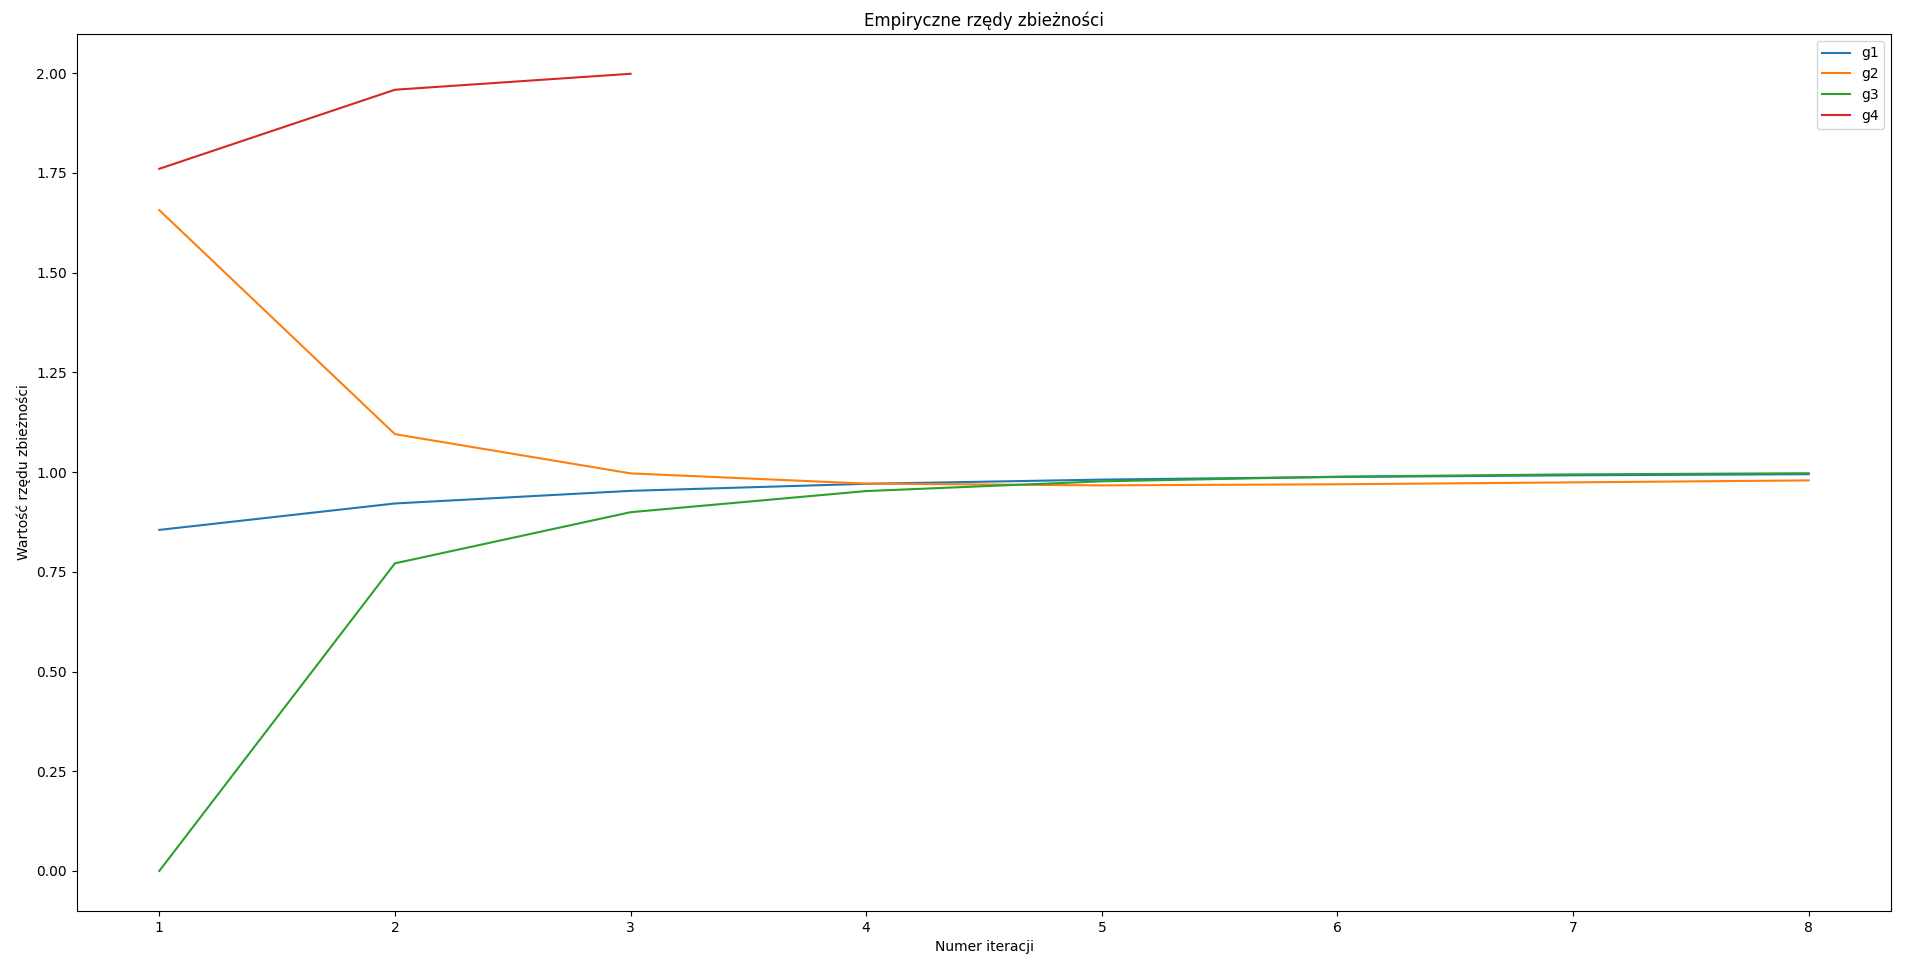
\includegraphics[scale = 0.3]{wykres1.png}
	\end{figure}


	\newpage

	\subsection*{Błędy względne}

	Na podstawie obliczonych wartości stworzono wspólny wykres wartości bezwzględnych błędów względnych dla każdej z metod iteracyjnych w zależności od liczby iteracji. Na osi $y$ zastosowano skalę logarytmiczną.

	\begin{figure}[h]
		\centering
		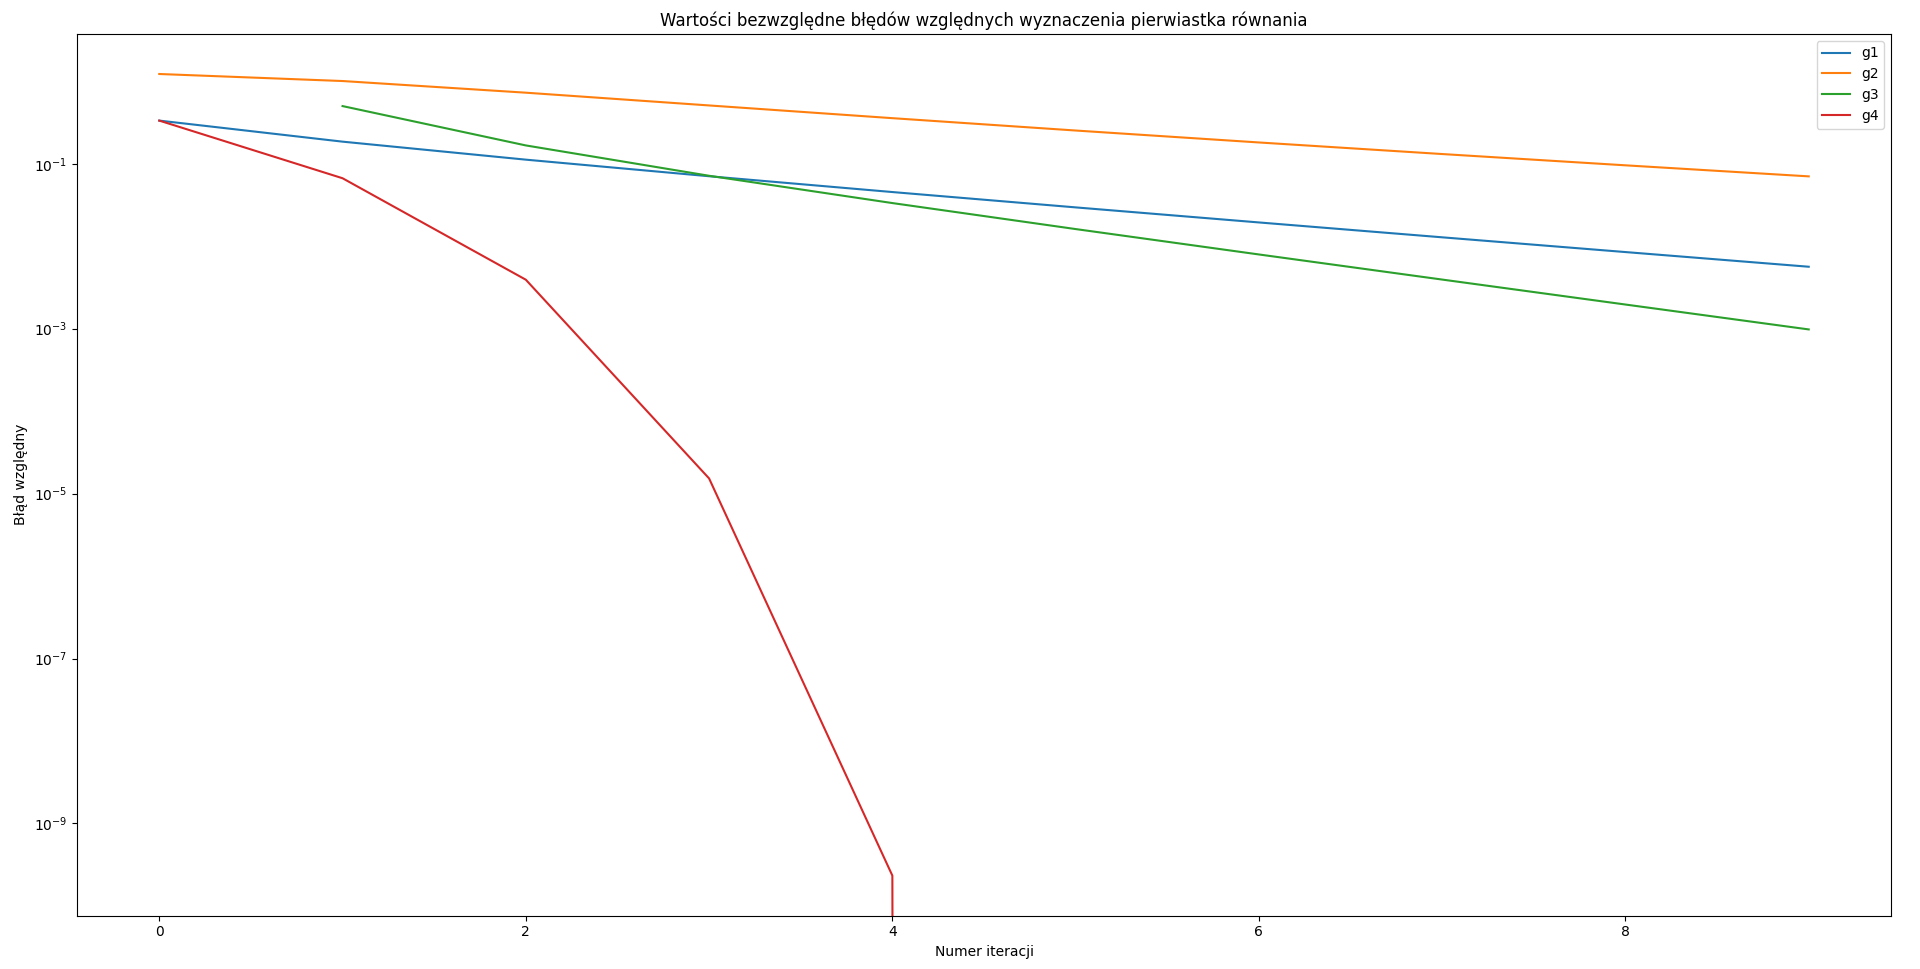
\includegraphics[scale = 0.3]{wykres2.png}
	\end{figure}



	\section*{Zadanie 2}
	
	\subsection*{Opis problemu}

	Celem zadania było napisanie schematów iteracji według metody Newtona dla każdego z następujących równań nieliniowych:
	
	\begin{equation}
		x^3 - 2x -5 = 0
	\end{equation}

	\begin{equation}
		e^{-x} = x
	\end{equation}

	\begin{equation}
		x \sin x = 1
	\end{equation}

	\subsection*{Wyznaczanie schematów}

	W celu wykonania zadania ustalono wzory funkcji $f_i$ odpowiadających odpowiednim danym równaniom:

	\begin{equation}
		f_1(x) = x^3 - 2x -5
	\end{equation}

	\begin{equation}
		f_2(x) = e^{-x} - x
	\end{equation}

	\begin{equation}
		f_3(x) = x \sin x - 1
	\end{equation}


	W kolejnym kroku wyprowadzono wzory na pierwsze pochodne powyższych funkcji:

	\begin{equation}
		f_1'(x) = 3x^2 - 2
	\end{equation}

	\begin{equation}
		f_2'(x) = -e^{-x} - 1
	\end{equation}

	\begin{equation}
		f_3'(x) = \sin x + x \cos x
	\end{equation}

	Korzystając ze wzoru:

	\begin{equation}
		x_{k+1} = x_k - \frac{f(x_k)}{f'(x_k)} 
	\end{equation}

	Wyznaczono funkcje $g_i(x_k)$ odpowiadające funkcjom $f_i(x)$ definiujące szukane schematy iteracyjne według metody Newtona:

	\begin{equation}
		g_1(x) = x - \frac{x^3 - 2x -5}{3x^2 - 2} = \frac{2x^3+5}{3x^2-2}
	\end{equation}

	\begin{equation}
		g_2(x) = x - \frac{e^{-x} - x}{-e^{-x} - 1} = \frac{(x+1) \cdot e^{-x}}{e^{-x} + 1}
	\end{equation}

	\begin{equation}
		g_3(x) = x - \frac{x \sin x - 1}{\sin x + x \cos x} = \frac{x^2 \cdot \cos x + 1}{x \cos x + \sin x}
	\end{equation}

	\subsection*{Dokładność}

	Wiedząc, że $x_0$ jest przybliżeniem pierwiastka z dokładnością 4 bitów, aby osiągnąć 24 bitową dokładność należy wykonać 2 iteracje. Wynika to z tego, że metoda Newtona rząd zbieżności kwadratowy, co oznacza, że z każdą iteracją, liczba ustalanych bitów wzrasta dwukrotnie. Oznacza to, że skoro początkowo $x_0$ miało dokładność 4 bitów, to po pierwszej iteracji miało dokładność 12 bitów (+8 bitów), a po drugiej już 28 (+16 bitów). Analogicznie aby mieć dokładność 53 bitów wystarczy wykonać jeszcze jedną iterację (łącznie 3), ponieważ po niej dokładność będzie wynosiła 60 bitów (+32 bity).


	\newpage


	\section*{Zadanie 3}

	\subsection*{Opis problemu}

	Celem zadania było napisanie schematu iteracji według metody Newtona dla następującego układu równań nieliniowych:

	\begin{equation}
		\systeme{x^2+y^2 = 1, x^2 - y = 0}
	\end{equation}

	\subsection*{Wyprowadzenie schematu}

	Z drugiego równania mamy:

	\begin{equation}
		x^2 = y
	\end{equation}

	Zatem podstawiając do pierwszego równania mamy:

	\begin{equation}
		y^2 +y - 1 = 0
	\end{equation}

	Zapiszmy:

	\begin{equation}
		f(y) = y^2 + y - 1
	\end{equation}

	Zatem:

	\begin{equation}
		f'(y) = 2y + 1
	\end{equation}

	Zatem korzystając z zależności (17), dostajemy;

	\begin{equation}
		g(x) = x - \frac{x^2 + x - 1}{2x+1} = \frac{x^2+1}{2x+1}
	\end{equation}

	Na tej podstawie napisano program w Pythonie wyznaczający miejsce zerowe funcji $f(y)$. Aby otrzymać rozwiązanie na $x$, należy spierwiastkować otrzymane $y_0$ (zgodnie z równaniem (22)). Otrzyame wyniki w zależności od liczby iteracji:

	\begin{center}
		\begin{tabular}{c|c|c}
  			\hline 
  			liczba iteracji & $x$ & $y$\\
  			\hline
  			$0$ & $0.0$ & $0.0$\\
  			$1$ & $\pm 1.0$ & $1.0$\\
  			$2$ & $\pm 0.816496580927726$ & $0.6666666666666666$\\
			$3$ & $\pm 0.7867957924694432$ & $0.6190476190476191$\\
  			$4$ & $\pm 0.7861516697315358$ & $0.6180344478216818$\\
  			$5$ & $\pm 0.7861513777574832$ & $0.6180339887499892$\\
			$6$ & $\pm 0.7861513777574233$ & $0.6180339887498949$\\
  			$7$ & $\pm 0.7861513777574233$ & $0.6180339887498948$\\
  			$8$ & $\pm 0.7861513777574233$ & $0.6180339887498948$\\
			$9$ & $\pm 0.7861513777574233$ & $0.6180339887498948$\\
		\end{tabular} 
		
	\end{center}	

	Wartości dokładne rozwiązania tego równania wynoszą:

	\begin{equation}
		x = \pm \sqrt{\frac{\sqrt{5}}{2} - \frac{1}{2}} \approx \pm 0,786151377
	\end{equation}

	\begin{equation}
		y = \frac{\sqrt{5}}{2} - \frac{1}{2} \approx 0,6118033988
	\end{equation}


	Wyniki z tabeli pokrywają się z wynikami otrzymanymi przy użyciu kalkulatora, co pozwala przypuszczać, że obliczania zostały wykonane prawidłowo. 

	Na podstawie obliczonych danych stworzono wykres błędu względnego $y$ znalezionego metodą Newtona w zależności od liczby iteracji. Na osi $y$ została zastosowana skala logarytmiczna.


	\begin{figure}[h]
		\centering
		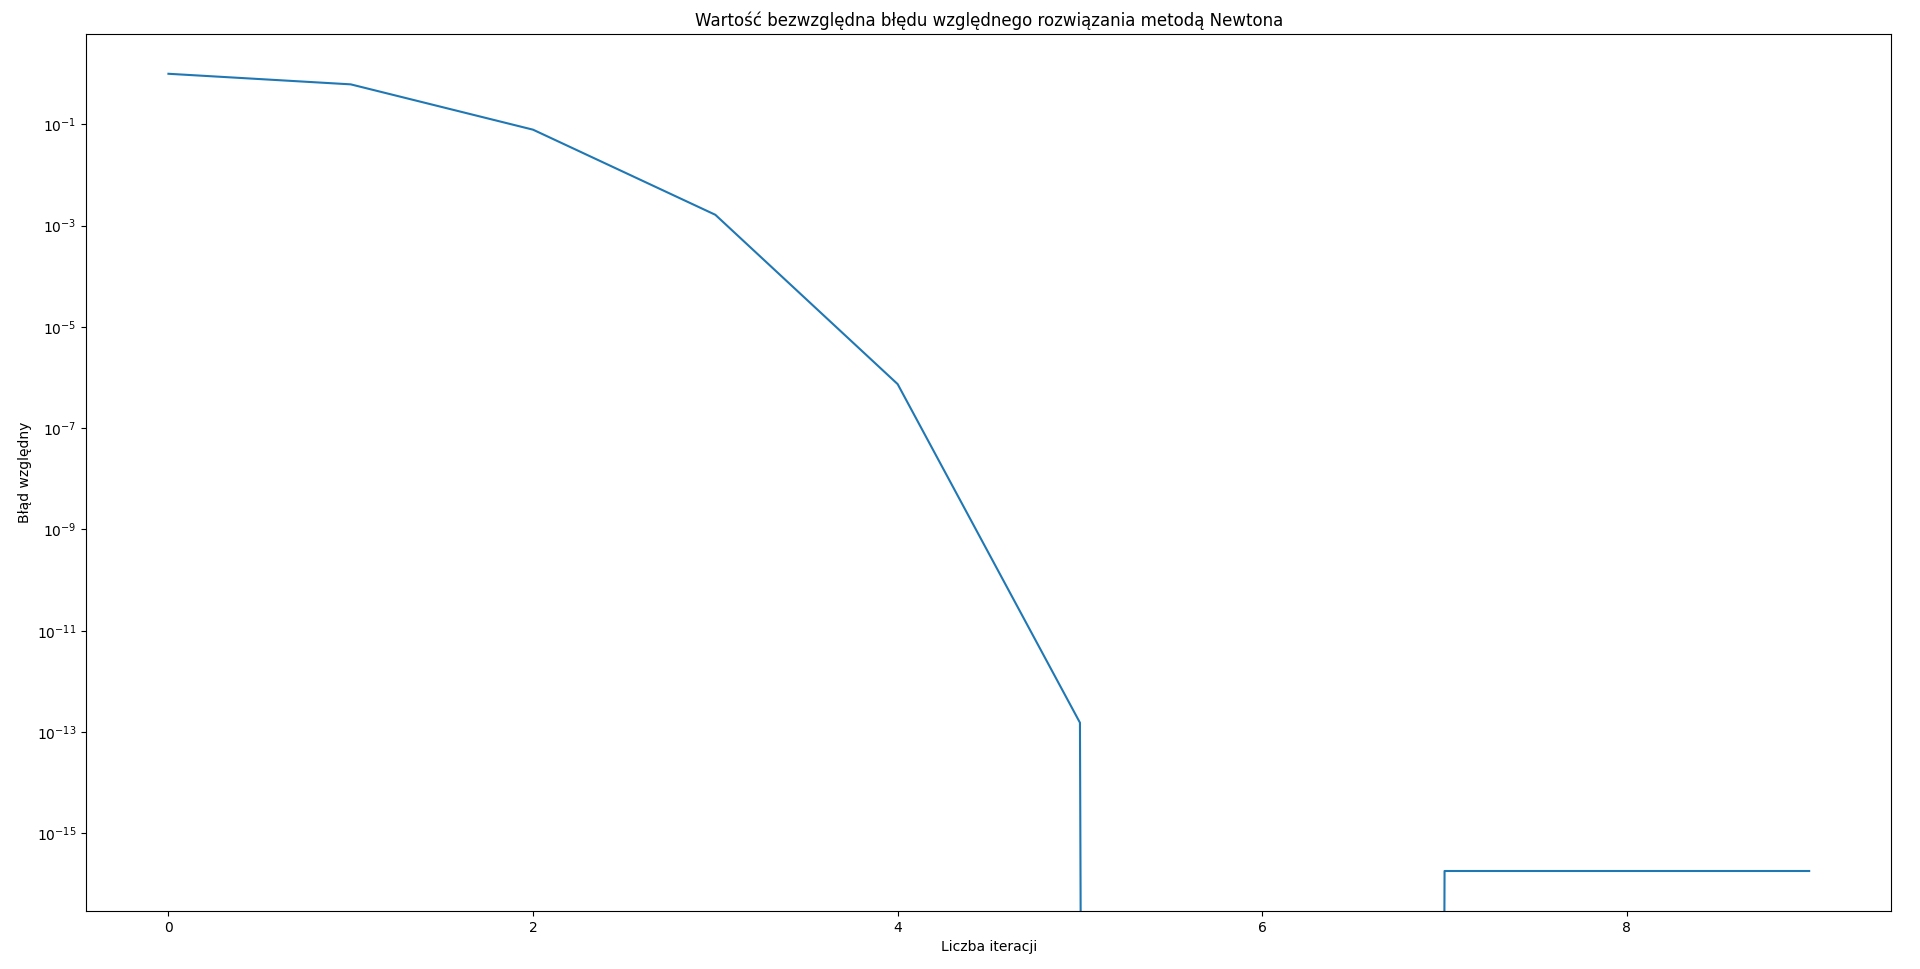
\includegraphics[scale = 0.3]{wykres3.png}
	\end{figure}

	Na wykresie można zauważyć moment, w którym błąd numeryczny przeważa nad błędem metody (około 7 iteracji).



	



	
	
	
	
	
	
	
	
	
\end{document}